\hypertarget{mtk__bc__desc__1d_8cc}{\section{src/mtk\+\_\+bc\+\_\+desc\+\_\+1d.cc File Reference}
\label{mtk__bc__desc__1d_8cc}\index{src/mtk\+\_\+bc\+\_\+desc\+\_\+1d.\+cc@{src/mtk\+\_\+bc\+\_\+desc\+\_\+1d.\+cc}}
}


Enforces boundary conditions in either the operator or the grid.  


{\ttfamily \#include \char`\"{}mtk\+\_\+tools.\+h\char`\"{}}\\*
{\ttfamily \#include \char`\"{}mtk\+\_\+bc\+\_\+desc\+\_\+1d.\+h\char`\"{}}\\*
Include dependency graph for mtk\+\_\+bc\+\_\+desc\+\_\+1d.\+cc\+:\nopagebreak
\begin{figure}[H]
\begin{center}
\leavevmode
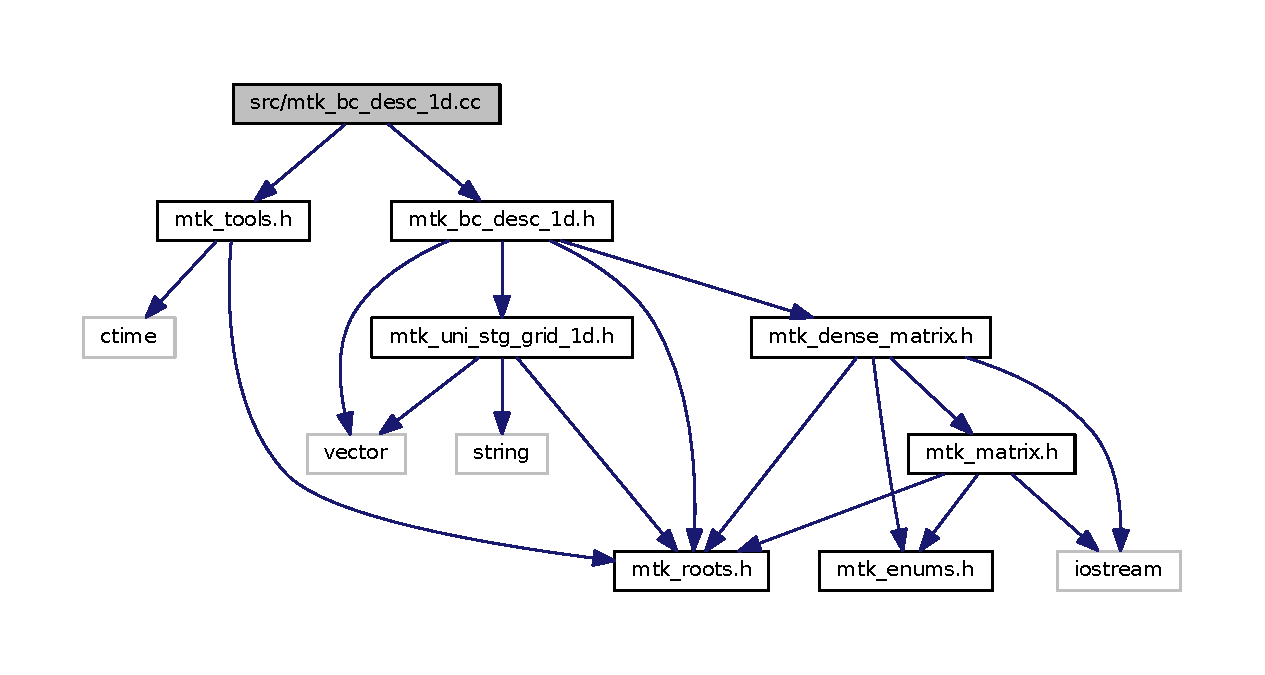
\includegraphics[width=350pt]{mtk__bc__desc__1d_8cc__incl}
\end{center}
\end{figure}


\subsection{Detailed Description}
This class presents an interface for the user to specify boundary conditions on 1\+D mimetic operators and the grids they are acting on.

\begin{DoxyAuthor}{Author}
\+: Eduardo J. Sanchez (ejspeiro) -\/ esanchez at mail dot sdsu dot edu 
\end{DoxyAuthor}


Definition in file \hyperlink{mtk__bc__desc__1d_8cc_source}{mtk\+\_\+bc\+\_\+desc\+\_\+1d.\+cc}.

